% answers.tex —— 2013 年·广东卷·理科 · 参考答案与详细解析片段
% 由 tools/generate_projects.py 依来源总账自 2013/2013_数学真题_广东理_试题.md + 2013/2013_数学真题_广东理_解析正文.md + 2013/2013_数学真题_广东理_答案要点.md 生成，勿手改（改源 MD 后重跑）


\begin{answer}
\gksolhead{1}{}

\textbf{题目}：

设集合 $M=\{x\mid x^2+2x=0,\ x\in\mathbf R\}$，$N=\{x\mid x^2-2x=0,\ x\in\mathbf R\}$，则 $M\cup N=$\mbox{（　　）}

（A）$\{0\}$；（B）$\{0,2\}$；（C）$\{-2,0\}$；（D）$\{-2,0,2\}$。

\Needspace{4\baselineskip}
\textbf{解析}
\Needspace{5\baselineskip}
由 $x^2+2x=x(x+2)=0$ 得
\nopagebreak[4]
\[M=\{-2,0\};\]
\Needspace{5\baselineskip}
由 $x^2-2x=x(x-2)=0$ 得
\nopagebreak[4]
\[N=\{0,2\}.\]
\Needspace{5\baselineskip}
因此
\nopagebreak[4]
\[M\cup N=\{-2,0,2\}.\]
选 D。

\gkanswer{答案：D。$M=\{-2,0\}$，$N=\{0,2\}$，故 $M\cup N=\{-2,0,2\}$。}

\end{answer}
\begin{answer}
\gksolhead{2}{}

\textbf{题目}：

定义域为 $\mathbf R$ 的四个函数 $y=x^3$，$y=2^x$，$y=x^2+1$，$y=2\sin x$ 中，奇函数的个数是\mbox{（　　）}

（A）$4$；（B）$3$；（C）$2$；（D）$1$。

\Needspace{4\baselineskip}
\textbf{解析}
四个函数的定义域均为 $\mathbf R$，关于原点对称。

\begin{itemize}
\item $y=x^3$：$(-x)^3=-x^3$，是奇函数；
\item $y=2^x$：$2^{-x}=\dfrac1{2^x}\neq -2^x$，且 $2^{-x}\neq 2^x$，非奇非偶；
\item $y=x^2+1$：$(-x)^2+1=x^2+1$，是偶函数；
\item $y=2\sin x$：$2\sin(-x)=-2\sin x$，是奇函数。
\end{itemize}

奇函数共有 $2$ 个。选 C。

\gkanswer{答案：C。$y=x^3$ 与 $y=2\sin x$ 是奇函数，$y=2^x$ 非奇非偶，$y=x^2+1$ 是偶函数，共 $2$ 个。}

\end{answer}
\begin{answer}
\gksolhead{3}{}

\textbf{题目}：

若复数 $z$ 满足 $\mathrm iz=2+4\mathrm i$，则在复平面内，$z$ 对应的点的坐标是\mbox{（　　）}

（A）$(2,4)$；（B）$(2,-4)$；（C）$(4,-2)$；（D）$(4,2)$。

\Needspace{4\baselineskip}
\textbf{解析}
\Needspace{5\baselineskip}
由 $\mathrm iz=2+4\mathrm i$，两边同乘 $-\mathrm i$（即除以 $\mathrm i$）：
\nopagebreak[4]
\[z=\frac{2+4\mathrm i}{\mathrm i}=(2+4\mathrm i)(-\mathrm i)=4-2\mathrm i.\]
所以 $z$ 对应的点为 $(4,-2)$。选 C。

\gkanswer{答案：C。$z=\dfrac{2+4\mathrm i}{\mathrm i}=4-2\mathrm i$，对应点 $(4,-2)$。}

\end{answer}
\begin{answer}
\gksolhead{4}{}

\textbf{题目}：

已知离散型随机变量 $X$ 的分布列为

\begin{center}
\begin{tabular}{llll}
\toprule
$X$ & $1$ & $2$ & $3$ \\
\midrule
$P$ & $\dfrac35$ & $\dfrac3{10}$ & $\dfrac1{10}$ \\
\bottomrule
\end{tabular}
\end{center}

则 $X$ 的数学期望 $E(X)=$\mbox{（　　）}

（A）$\dfrac32$；（B）$2$；（C）$\dfrac52$；（D）$3$。

\Needspace{4\baselineskip}
\textbf{解析}
\Needspace{5\baselineskip}
由分布列，
\nopagebreak[4]
\[\begin{aligned}
E(X)&=1\cdot\frac35+2\cdot\frac3{10}+3\cdot\frac1{10}\\
&=\frac35+\frac35+\frac3{10}\\
&=\frac{6+6+3}{10}=\frac{15}{10}=\frac32.
\end{aligned}\]
选 A。

\gkanswer{答案：A。$E(X)=1\cdot\dfrac35+2\cdot\dfrac3{10}+3\cdot\dfrac1{10}=\dfrac32$。}

\end{answer}
\begin{answer}
\gksolhead{5}{}

\textbf{题目}：

某四棱台的三视图如图所示，则该四棱台的体积是\mbox{（　　）}
\nopagebreak[4]
\begin{center}% 2013 年广东卷理科第 5 题：四棱台的三视图。
% 来源 PDF：普通高考/2013/2013广东理.pdf，第 1 页（印面 803）左栏。
% 正视图、侧视图均为上底 1、下底 2、高 2 的直角梯形；俯视图为边长 2 的正方形，
% 上底面投影为左上角边长 1 的正方形。
\begin{tikzpicture}[semithick, font=\small, >=Stealth]
  \useasboundingbox (-1.0,-6.05) rectangle (6.4,2.9);
  % 正视图
  \draw (0,0) -- (2,0) -- (1,2) -- (0,2) -- cycle;
  \draw[<->] (0,2.42) -- (1,2.42) node[midway,above] {$1$};
  \draw[<->] (0,-0.42) -- (2,-0.42) node[midway,below] {$2$};
  \draw[<->] (-0.42,0) -- (-0.42,2) node[midway,left] {$2$};
  \draw (0,2.42) -- (0,2.05);
  \draw (1,2.42) -- (1,2.05);
  \node at (1,-1.05) {正视图};
  % 侧视图
  \begin{scope}[xshift=3.55cm]
    \draw (0,0) -- (2,0) -- (1,2) -- (0,2) -- cycle;
    \node at (1,-1.05) {侧视图};
  \end{scope}
  % 俯视图
  \begin{scope}[yshift=-6.0cm]
    \draw (0,0) rectangle (2,2);
    \draw (0,1) -- (1,1) -- (1,2);
    \draw (1,1) -- (2,0);
    \draw[<->] (-0.42,1) -- (-0.42,2) node[midway,left] {$1$};
    \draw[<->] (-0.42,0) -- (-0.42,1) node[midway,left] {$1$};
    \node at (1,-0.55) {俯视图};
  \end{scope}
\end{tikzpicture}
\end{center}
\nopagebreak[4]
（A）$4$；（B）$\dfrac{14}{3}$；（C）$\dfrac{16}{3}$；（D）$6$。

\Needspace{4\baselineskip}
\textbf{解析}
\Needspace{5\baselineskip}
由三视图，四棱台的上、下底面都是正方形：上底边长 $a=1$，下底边长 $b=2$，高 $h=2$。棱台体积公式为
\nopagebreak[4]
\[V=\frac h3\left(S_{\text{\text{上}}}+S_{\text{\text{下}}}+\sqrt{S_{\text{\text{上}}}S_{\text{\text{下}}}}\right).\]
\Needspace{5\baselineskip}
代入 $S_{\text{\text{上}}}=1$，$S_{\text{\text{下}}}=4$：
\nopagebreak[4]
\[V=\frac23\left(1+4+\sqrt{1\cdot4}\right)=\frac23(1+4+2)=\frac{14}{3}.\]
选 B。

\gkanswer{答案：B。三视图给出上底边长 $1$、下底边长 $2$、高 $2$，$V=\dfrac23(1+4+2)=\dfrac{14}{3}$。}

\end{answer}
\begin{answer}
\gksolhead{6}{}

\textbf{题目}：

设 $m$，$n$ 是两条不同的直线，$\alpha$，$\beta$ 是两个不同的平面，下列命题中正确的是\mbox{（　　）}

（A）若 $\alpha\perp\beta$，$m\subset\alpha$，$n\subset\beta$，则 $m\perp n$；（B）若 $\alpha\parallel\beta$，$m\subset\alpha$，$n\subset\beta$，则 $m\parallel n$；（C）若 $m\perp n$，$m\subset\alpha$，$n\subset\beta$，则 $\alpha\perp\beta$；（D）若 $m\perp\alpha$，$m\parallel n$，$n\parallel\beta$，则 $\alpha\perp\beta$。

\Needspace{4\baselineskip}
\textbf{解析}
逐一判断：

（A）若 $\alpha\perp\beta$，$m\subset\alpha$，$n\subset\beta$，$m$ 与 $n$ 可能平行。例如取 $\alpha$ 为 $x=0$ 平面、$\beta$ 为 $y=0$ 平面，$m$ 为 $\alpha$ 内的 $z$ 轴，$n$ 为 $\beta$ 内平行于 $z$ 轴的直线，则 $m\parallel n$，并不垂直。故 A 错。

（B）若 $\alpha\parallel\beta$，$m\subset\alpha$，$n\subset\beta$，$m$ 与 $n$ 可能异面。例如取 $\alpha:z=0$、$\beta:z=1$，$m$ 为 $x$ 轴，$n$ 为 $\beta$ 内平行于 $y$ 轴的直线，二者异面。故 B 错。

（C）若 $m\perp n$，$m\subset\alpha$，$n\subset\beta$，不能推出 $\alpha\perp\beta$。例如取 $\alpha\parallel\beta$，$m$ 为 $\alpha$ 内的 $x$ 轴，$n$ 为 $\beta$ 内平行于 $y$ 轴的直线，则 $m\perp n$ 但 $\alpha\parallel\beta$。故 C 错。

（D）由 $m\parallel n$、$m\perp\alpha$ 得 $n\perp\alpha$。又 $n\parallel\beta$，故可在 $\beta$ 内取一条与 $n$ 平行的直线 $l$，于是 $l\perp\alpha$。平面 $\beta$ 含有垂直于平面 $\alpha$ 的直线，所以 $\alpha\perp\beta$。故 D 正确。

选 D。

\gkanswer{答案：D。由 $m\perp\alpha$、$m\parallel n$ 得 $n\perp\alpha$，又 $n\parallel\beta$，故 $\alpha\perp\beta$；其余三项均可举反例。}

\end{answer}
\begin{answer}
\gksolhead{7}{}

\textbf{题目}：

已知中心在原点的双曲线 $C$ 的右焦点为 $F(3,0)$，离心率等于 $\dfrac32$，则 $C$ 的方程是\mbox{（　　）}

（A）$\dfrac{x^2}{4}-\dfrac{y^2}{\sqrt5}=1$；（B）$\dfrac{x^2}{4}-\dfrac{y^2}{5}=1$；（C）$\dfrac{x^2}{2}-\dfrac{y^2}{5}=1$；（D）$\dfrac{x^2}{2}-\dfrac{y^2}{\sqrt5}=1$。

\Needspace{4\baselineskip}
\textbf{解析}
\Needspace{5\baselineskip}
设双曲线方程为 $\dfrac{x^2}{a^2}-\dfrac{y^2}{b^2}=1$（$a>0$，$b>0$）。右焦点为 $(c,0)$，则 $c=3$。离心率
\nopagebreak[4]
\[e=\frac ca=\frac32\Longrightarrow a=2.\]
\Needspace{5\baselineskip}
于是
\nopagebreak[4]
\[b^2=c^2-a^2=9-4=5.\]
\Needspace{5\baselineskip}
故方程为
\nopagebreak[4]
\[\frac{x^2}{4}-\frac{y^2}{5}=1.\]
选 B。

\gkanswer{答案：B。$c=3$，$e=\dfrac ca=\dfrac32$，故 $a=2$，$b^2=c^2-a^2=5$，方程为 $\dfrac{x^2}{4}-\dfrac{y^2}{5}=1$。}

\end{answer}
\begin{answer}
\gksolhead{8}{}

\textbf{题目}：

设整数 $n\geqslant4$，集合 $X=\{1,2,3,\cdots,n\}$。令集合 $S=\{(x,y,z)\mid x,y,z\in X,\ \text{\text{且三条件}}\ x<y<z,\ y<z<x,\ z<x<y\ \text{\text{恰有一个成立}}\}$，若 $(x,y,z)$ 和 $(z,w,x)$ 都在 $S$ 中，则下列选项正确的是\mbox{（　　）}

（A）$(y,z,w)\in S$，$(x,y,w)\notin S$；（B）$(y,z,w)\in S$，$(x,y,w)\in S$；（C）$(y,z,w)\notin S$，$(x,y,w)\in S$；（D）$(y,z,w)\notin S$，$(x,y,w)\notin S$。

\Needspace{4\baselineskip}
\textbf{解析}
$S$ 中的三个数互不相同，且三元组在数值递增的循环次序中排列。也就是说，把 $x,y,z$ 按大小放在一个圆周上，$S$ 恰好选出按同一方向依次递增的三元组。

\Needspace{5\baselineskip}
由 $(x,y,z)\in S$，沿递增方向依次为 $x,y,z$；由 $(z,w,x)\in S$，从 $z$ 出发沿递增方向依次为 $z,w,x$。合起来，四个数沿递增方向的循环次序为
\nopagebreak[4]
\[x\to y\to z\to w\to x.\]
\Needspace{5\baselineskip}
于是从 $y$ 出发依次得到 $y,z,w$，从 $x$ 出发依次得到 $x,y,w$，二者都按递增循环次序排列，故
\nopagebreak[4]
\[(y,z,w)\in S,\qquad (x,y,w)\in S.\]
选 B。

\gkanswer{答案：B。$S$ 表示三数按递增循环次序排列；由两已知三元组合得 $x,y,z,w$ 的循环次序，故 $(y,z,w)$ 与 $(x,y,w)$ 都在 $S$ 中。}

\end{answer}
\begin{answer}
\gksolhead{9}{}

\textbf{题目}：

不等式 $x^2+x-2<0$ 的解集为\gkblank{}。

\Needspace{4\baselineskip}
\textbf{解析}
\Needspace{5\baselineskip}
因式分解：
\nopagebreak[4]
\[x^2+x-2=(x+2)(x-1)<0.\]
\Needspace{5\baselineskip}
二次项系数为正，故解在两根之间：
\nopagebreak[4]
\[-2<x<1.\]
解集为 $\{x\mid -2<x<1\}$。

\gkanswer{答案：$\{x\mid -2<x<1\}$。$(x+2)(x-1)<0$，故 $-2<x<1$。}

\end{answer}
\begin{answer}
\gksolhead{10}{}

\textbf{题目}：

若曲线 $y=kx+\ln x$ 在点 $(1,k)$ 处的切线平行于 $x$ 轴，则 $k=$\gkblank{}。

\Needspace{4\baselineskip}
\textbf{解析}
\Needspace{5\baselineskip}
函数的定义域为 $x>0$，且
\nopagebreak[4]
\[y'=k+\frac1x.\]
\Needspace{5\baselineskip}
曲线在点 $(1,k)$ 处的切线斜率为
\nopagebreak[4]
\[y'\big|_{x=1}=k+1.\]
\Needspace{5\baselineskip}
切线与 $x$ 轴平行，斜率为 $0$，故
\nopagebreak[4]
\[k+1=0\Longrightarrow k=-1.\]

\gkanswer{答案：$-1$。$y'=k+\dfrac1x$，在 $x=1$ 处 $k+1=0$。}

\end{answer}
\begin{answer}
\gksolhead{11}{}

\textbf{题目}：

执行如图所示的程序框图，若输入 $n$ 的值为 $4$，则输出 $s$ 的值为\gkblank{}。
\nopagebreak[4]
\begin{center}% 2013 年广东卷理科第 11 题：输出 s 的程序框图。
% 来源 PDF：普通高考/2013/2013广东理.pdf，第 1 页（印面 803）中栏。
% 流程：开始 → 输入 n → i=1,s=1 → i≤n? 是：s=s+(i−1)，i=i+1，回到判断；
% 否：输出 s → 结束。原卷循环体为 s=s+(i−1)，非平方。
\begin{tikzpicture}[semithick, >=Stealth, font=\small,
  block/.style={draw, minimum width=3.1cm, minimum height=0.62cm, align=center},
  dec/.style={draw, diamond, aspect=2.6, inner sep=1pt, align=center},
  term/.style={draw, rounded corners=6pt, minimum width=1.4cm, minimum height=0.52cm},
  io/.style={draw, trapezium, trapezium left angle=70, trapezium right angle=110,
             minimum width=2.4cm, minimum height=0.62cm},
  arr/.style={->}]
  \useasboundingbox (-2.9,-6.2) rectangle (5.0,0.6);
  \node (start) [term] at (0,0) {开始};
  \node (input) [io]   at (0,-1.05) {输入 $n$};
  \node (init)  [block] at (0,-2.1) {$i=1,\ s=1$};
  \node (dec)   [dec]  at (0,-3.35) {$i\le n$?};
  \node (body)  [block] at (0,-4.75) {$s=s+(i-1)$};
  \node (inc)   [block] at (0,-5.85) {$i=i+1$};
  \node (out)   [io]   at (3.55,-3.35) {输出 $s$};
  \node (end)   [term] at (3.55,-4.75) {结束};
  \draw[arr] (start) -- (input);
  \draw[arr] (input) -- (init);
  \draw[arr] (init) -- (dec);
  \draw[arr] (dec) -- node[left, xshift=-1pt] {是} (body);
  \draw[arr] (body) -- (inc);
  \draw[arr] (dec.east) -- node[above] {否} (out.west);
  \draw[arr] (out) -- (end);
  \draw[arr] (inc.west) -- (-2.2,-5.85) -- (-2.2,-2.55) -- (0,-2.55);
\end{tikzpicture}
\end{center}
\nopagebreak[4]
\Needspace{4\baselineskip}
\textbf{解析}
\Needspace{5\baselineskip}
初值 $i=1$，$s=1$。每轮先判断 $i\leqslant n$，为真则执行
\nopagebreak[4]
\[s=s+(i-1),\qquad i=i+1,\]
再回到判断。取 $n=4$，逐轮计算：

\begin{center}
\begin{tabular}{llll}
\toprule
判断时的 $i$ & $i\leqslant4$ & 执行后 $s$ & 执行后 $i$ \\
\midrule
$1$ & 真 & $1+(1-1)=1$ & $2$ \\
$2$ & 真 & $1+(2-1)=2$ & $3$ \\
$3$ & 真 & $2+(3-1)=4$ & $4$ \\
$4$ & 真 & $4+(4-1)=7$ & $5$ \\
$5$ & 假 & 不再执行 & 输出 $s$ \\
\bottomrule
\end{tabular}
\end{center}

\Needspace{5\baselineskip}
故输出
\nopagebreak[4]
\[s=1+0+1+2+3=7.\]

\gkanswer{答案：$7$。循环体为 $s=s+(i-1)$，依次累加 $0,1,2,3$ 到初值 $1$ 上。}

\end{answer}
\begin{answer}
\gksolhead{12}{}

\textbf{题目}：

在等差数列 $\{a_n\}$ 中，已知 $a_3+a_8=10$，则 $3a_5+a_7=$\gkblank{}。

\Needspace{4\baselineskip}
\textbf{解析}
\Needspace{5\baselineskip}
设等差数列的首项为 $a_1$，公差为 $d$。由
\nopagebreak[4]
\[a_3+a_8=(a_1+2d)+(a_1+7d)=2a_1+9d=10.\]
\Needspace{5\baselineskip}
而
\nopagebreak[4]
\[\begin{aligned}
3a_5+a_7&=3(a_1+4d)+(a_1+6d)\\
&=4a_1+18d\\
&=2(2a_1+9d)\\
&=2\times10=20.
\end{aligned}\]

\gkanswer{答案：$20$。$a_3+a_8=2a_1+9d=10$，而 $3a_5+a_7=4a_1+18d=2(2a_1+9d)=20$。}

\end{answer}
\begin{answer}
\gksolhead{13}{}

\textbf{题目}：

给定区域 $D:\begin{cases}x+4y\geqslant4,\\ x+y\leqslant4,\\ x\geqslant0,\end{cases}$ 令点集 $T=\{(x_0,y_0)\in D\mid x_0,y_0\in\mathbf Z,\ (x_0,y_0)\ \text{\text{是}}\ z=x+y\ \text{\text{在}}\ D\ \text{\text{上取得最大值或最小值的点}}\}$，则 $T$ 中的点共确定\gkblank{}条不同的直线。

\Needspace{4\baselineskip}
\textbf{解析}
\Needspace{5\baselineskip}
区域 $D$ 由三条边界围成，其顶点为
\nopagebreak[4]
\[(0,1),\qquad (4,0),\qquad (0,4).\]
目标函数 $z=x+y$ 在这三点处的值分别为 $1,4,4$，故最小值为 $1$，最大值为 $4$。

\Needspace{5\baselineskip}
最小值的点：在 $x+y=1$ 上，须同时满足 $x+4y\geqslant4$。以 $y=1-x$ 代入：
\nopagebreak[4]
\[x+4(1-x)\geqslant4\Longrightarrow 4-3x\geqslant4\Longrightarrow x\leqslant0.\]
又 $x\geqslant0$，故 $x=0$，$y=1$，即 $(0,1)$。

\Needspace{5\baselineskip}
最大值的点：在 $x+y=4$ 上，整数点有
\nopagebreak[4]
\[(0,4),(1,3),(2,2),(3,1),(4,0),\]
\Needspace{5\baselineskip}
它们都满足 $x+4y\geqslant4$。故
\nopagebreak[4]
\[T=\{(0,1),(0,4),(1,3),(2,2),(3,1),(4,0)\}.\]

\Needspace{5\baselineskip}
其中 $(0,4),(1,3),(2,2),(3,1),(4,0)$ 五点共线于 $x+y=4$，确定 $1$ 条直线。点 $(0,1)$ 与这五点分别连线，斜率依次为
\nopagebreak[4]
\[\text{\text{不存在}},\quad 2,\quad \frac12,\quad 0,\quad -\frac14,\]
\Needspace{5\baselineskip}
五条直线互不相同。因此 $T$ 中的点共确定
\nopagebreak[4]
\[1+5=6\]
条不同的直线。

\gkanswer{答案：$6$。$T=\{(0,1),(0,4),(1,3),(2,2),(3,1),(4,0)\}$，其中五个最大值点在 $x+y=4$ 上，另一点与它们各连一条，共 $1+5=6$ 条。}

\end{answer}
\begin{answer}
\gksolhead{14}{}

\textbf{题目}：

（选做）已知曲线 $C$ 的参数方程为 $\begin{cases}x=\sqrt2\cos t,\\ y=\sqrt2\sin t,\end{cases}$（$t$ 为参数），$C$ 在点 $(1,1)$ 处的切线为 $l$，以坐标原点为极点，$x$ 轴的正半轴为极轴建立极坐标系，则 $l$ 的极坐标方程为\gkblank{}。

\Needspace{4\baselineskip}
\textbf{解析}
\Needspace{5\baselineskip}
由参数方程
\nopagebreak[4]
\[x=\sqrt2\cos t,\qquad y=\sqrt2\sin t\]
\Needspace{5\baselineskip}
消去 $t$，得
\nopagebreak[4]
\[x^2+y^2=2,\]
\Needspace{5\baselineskip}
即曲线 $C$ 是以原点为圆心、$\sqrt2$ 为半径的圆。点 $(1,1)$ 在圆上，过该点的半径斜率为 $1$，故切线斜率为 $-1$。切线 $l$ 的方程为
\nopagebreak[4]
\[y-1=-(x-1)\Longrightarrow x+y=2.\]
\Needspace{5\baselineskip}
用 $x=\rho\cos\theta$，$y=\rho\sin\theta$ 代入，得极坐标方程
\nopagebreak[4]
\[\rho\cos\theta+\rho\sin\theta=2,\]
\Needspace{5\baselineskip}
即
\nopagebreak[4]
\[\rho(\cos\theta+\sin\theta)=2.\]

\gkanswer{答案：$\rho(\cos\theta+\sin\theta)=2$。圆为 $x^2+y^2=2$，在 $(1,1)$ 处的切线为 $x+y=2$。}

\end{answer}
\begin{answer}
\gksolhead{15}{}

\textbf{题目}：

（选做）如图，$AB$ 是圆 $O$ 的直径，点 $C$ 在圆 $O$ 上，延长 $BC$ 到 $D$ 使 $BC=CD$，过 $C$ 作圆 $O$ 的切线交 $AD$ 于 $E$。若 $AB=6$，$ED=2$，则 $BC=$\gkblank{}。
\nopagebreak[4]
\begin{center}% 2013 年广东卷理科第 15 题：圆 O 的直径 AB，C 在圆上，BC=CD，
% 过 C 的切线与 AD 交于 E，AB=6，ED=2。
% 来源 PDF：普通高考/2013/2013广东理.pdf，第 1 页（印面 803）中栏下部。
% 按计算结果作图：半径 3，BC=2√3，AC=2√6，E 在 AD 上且 AE=4。
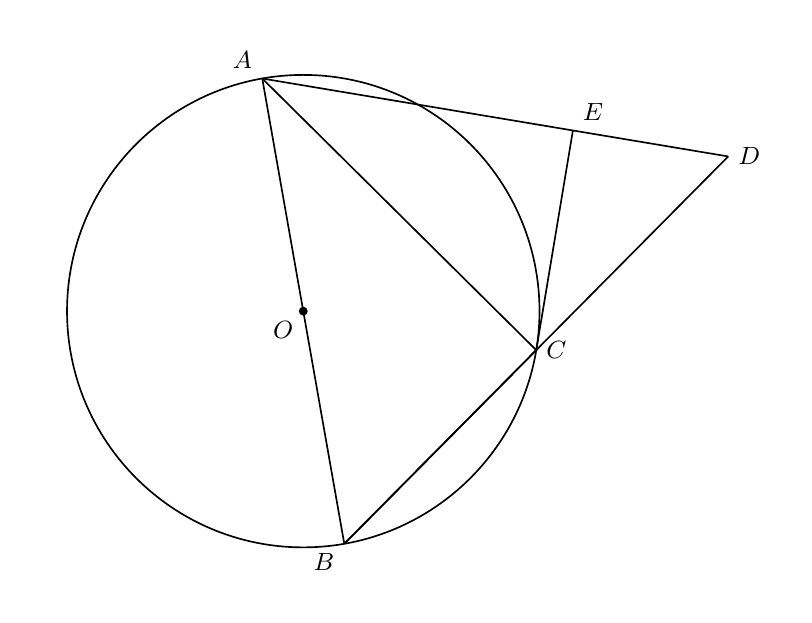
\begin{tikzpicture}[semithick, font=\small]
  \useasboundingbox (-3.5,-3.6) rectangle (6.1,3.6);
  \coordinate (O) at (0,0);
  \coordinate (A) at (-0.5209,2.9544);
  \coordinate (B) at (0.5209,-2.9544);
  \coordinate (C) at (2.9590,-0.4949);
  \coordinate (D) at (5.3971,1.9646);
  \coordinate (E) at (3.4245,2.2945);
  \draw (O) circle[radius=3];
  \draw (A) -- (B);
  \draw (A) -- (C) -- (B);
  \draw (B) -- (D);
  \draw (A) -- (D);
  \draw (C) -- (E);
  \fill (O) circle[radius=1.6pt];
  \node[above left] at (A) {$A$};
  \node[below left] at (B) {$B$};
  \node[right] at (C) {$C$};
  \node[right] at (D) {$D$};
  \node[above right] at (E) {$E$};
  \node[below left] at (O) {$O$};
\end{tikzpicture}
\end{center}
\nopagebreak[4]
\Needspace{4\baselineskip}
\textbf{解析}
\Needspace{5\baselineskip}
设 $BC=b$，$AC=h$。因为 $AB$ 是直径，所以
\nopagebreak[4]
\[\angle ACB=90^\circ,\]
\Needspace{5\baselineskip}
即 $AC\perp BC$。又 $C$ 是 $BD$ 的中点（$BC=CD$），故 $AC$ 是 $BD$ 的垂直平分线，从而
\nopagebreak[4]
\[AD=AB=6.\]
\Needspace{5\baselineskip}
由 $ED=2$，$E$ 在 $AD$ 上，得
\nopagebreak[4]
\[AE=AD-ED=6-2=4.\]

\Needspace{5\baselineskip}
取 $C$ 为原点，$CD$ 方向为 $x$ 轴正方向，则
\nopagebreak[4]
\[C=(0,0),\quad B=(b,0),\quad D=(-b,0),\quad A=(0,h).\]
\Needspace{5\baselineskip}
由 $AB=6$，
\nopagebreak[4]
\[b^2+h^2=36. \tag{1}\]

\Needspace{5\baselineskip}
圆以 $AB$ 为直径，圆心 $O=\left(\dfrac b2,\dfrac h2\right)$。过 $C$ 的切线与 $OC$ 垂直，而 $\overrightarrow{OC}=\left(\dfrac b2,\dfrac h2\right)$，故切线方程为
\nopagebreak[4]
\[bx+hy=0.\]

\Needspace{5\baselineskip}
点 $E$ 在 $AD$ 上且 $AE:ED=4:2=2:1$，所以
\nopagebreak[4]
\[E=A+\frac23(D-A)=\left(-\frac{2b}{3},\frac h3\right).\]
\Needspace{5\baselineskip}
因为 $E$ 在切线上，
\nopagebreak[4]
\[b\left(-\frac{2b}{3}\right)+h\cdot\frac h3=0
\Longrightarrow -2b^2+h^2=0
\Longrightarrow h^2=2b^2. \tag{2}\]
\Needspace{5\baselineskip}
将（2）代入（1）：
\nopagebreak[4]
\[b^2+2b^2=36\Longrightarrow 3b^2=36\Longrightarrow b^2=12.\]
\Needspace{5\baselineskip}
故
\nopagebreak[4]
\[BC=b=2\sqrt3.\]

\gkanswer{答案：$2\sqrt3$。设 $BC=b$，$AC=h$，由 $AD=AB=6$、$AE=4$ 及 $E$ 在切线上得 $h^2=2b^2$，结合 $b^2+h^2=36$ 得 $b=2\sqrt3$。}

\end{answer}
\begin{answer}
\gksolhead{16}{}

\textbf{题目}：

已知函数 $f(x)=\sqrt2\cos\left(x-\dfrac{\pi}{12}\right)$，$x\in\mathbf R$。

（1） 求 $f\left(-\dfrac{\pi}{6}\right)$ 的值；

（2） 若 $\cos\theta=\dfrac35$，$\theta\in\left(\dfrac{3\pi}{2},2\pi\right)$，求 $f\left(2\theta+\dfrac{\pi}{3}\right)$。

\Needspace{4\baselineskip}
\textbf{解析}
\Needspace{5\baselineskip}
\textbf{（1）}
\nopagebreak[4]
\[\begin{aligned}
f\left(-\frac{\pi}{6}\right)
&=\sqrt2\cos\left(-\frac{\pi}{6}-\frac{\pi}{12}\right)\\
&=\sqrt2\cos\left(-\frac{\pi}{4}\right)\\
&=\sqrt2\cdot\frac{\sqrt2}{2}=1.
\end{aligned}\]

\textbf{（2）}
\Needspace{5\baselineskip}
由 $\cos\theta=\dfrac35$ 且 $\theta\in\left(\dfrac{3\pi}{2},2\pi\right)$，知 $\sin\theta<0$，故
\nopagebreak[4]
\[\sin\theta=-\sqrt{1-\cos^2\theta}=-\sqrt{1-\frac9{25}}=-\frac45.\]
\Needspace{5\baselineskip}
于是
\nopagebreak[4]
\[\cos2\theta=2\cos^2\theta-1=2\cdot\frac9{25}-1=-\frac7{25},\]
\nopagebreak[4]
\[\sin2\theta=2\sin\theta\cos\theta=2\cdot\left(-\frac45\right)\cdot\frac35=-\frac{24}{25}.\]
\Needspace{5\baselineskip}
又
\nopagebreak[4]
\[\begin{aligned}
f\left(2\theta+\frac{\pi}{3}\right)
&=\sqrt2\cos\left(2\theta+\frac{\pi}{3}-\frac{\pi}{12}\right)\\
&=\sqrt2\cos\left(2\theta+\frac{\pi}{4}\right)\\
&=\sqrt2\left(\cos2\theta\cos\frac{\pi}{4}-\sin2\theta\sin\frac{\pi}{4}\right)\\
&=\cos2\theta-\sin2\theta\\
&=-\frac7{25}+\frac{24}{25}=\frac{17}{25}.
\end{aligned}\]

\gkanswer{答案（1）：$1$。$f\left(-\dfrac{\pi}{6}\right)=\sqrt2\cos\left(-\dfrac{\pi}{4}\right)=1$。}

\gkanswer{答案（2）：$\dfrac{17}{25}$。由 $\cos\theta=\dfrac35$、$\theta$ 在第四象限得 $\sin\theta=-\dfrac45$，再用二倍角公式计算。}

\end{answer}
\begin{answer}
\gksolhead{17}{}

\textbf{题目}：

某车间共有 $12$ 名工人，随机抽取 $6$ 名，他们某日加工零件个数的茎叶图如图所示，其中茎为十位数，叶为个位数。
\nopagebreak[4]
\begin{center}% 2013 年广东卷理科第 17 题：12 名工人日加工零件数的样本茎叶图。
% 来源 PDF：普通高考/2013/2013广东理.pdf，第 1 页（印面 803）右栏中部。
% 茎为十位数，叶为个位数：1|7 9；2|0 1 5；3|0。
\begin{tikzpicture}[semithick, font=\small]
  \useasboundingbox (-0.7,-1.0) rectangle (2.0,3.1);
  \draw (0,2.45) -- (0,-0.45);
  \node at (-0.35,2) {$1$};
  \node at (0.4,2) {$7$};
  \node at (0.95,2) {$9$};
  \node at (-0.35,1) {$2$};
  \node at (0.4,1) {$0$};
  \node at (0.95,1) {$1$};
  \node at (1.5,1) {$5$};
  \node at (-0.35,0) {$3$};
  \node at (0.4,0) {$0$};
\end{tikzpicture}
\end{center}
\nopagebreak[4]
（1） 根据茎叶图计算样本均值；

（2） 日加工零件个数大于样本均值的工人为优秀工人。根据茎叶图推断该车间 $12$ 名工人中有几名优秀工人？

（3） 从该车间 $12$ 名工人中，任取 $2$ 人，求恰有 $1$ 名优秀工人的概率。

\Needspace{4\baselineskip}
\textbf{解析}
\textbf{（1）}
\Needspace{5\baselineskip}
由茎叶图，$6$ 个数据为
\nopagebreak[4]
\[17,\ 19,\ 20,\ 21,\ 25,\ 30.\]
\Needspace{5\baselineskip}
样本均值
\nopagebreak[4]
\[\bar x=\frac{17+19+20+21+25+30}{6}=\frac{132}{6}=22.\]

\textbf{（2）}
\Needspace{5\baselineskip}
样本中大于 $22$ 的数据为 $25$ 和 $30$，共 $2$ 个，占样本的
\nopagebreak[4]
\[\frac26=\frac13.\]
\Needspace{5\baselineskip}
按此比例估计，该车间 $12$ 名工人中优秀工人约有
\nopagebreak[4]
\[12\times\frac13=4\]
名。

\textbf{（3）}
\Needspace{5\baselineskip}
由（2）估计该车间有 $4$ 名优秀工人、$8$ 名非优秀工人。从 $12$ 人中任取 $2$ 人，共有
\nopagebreak[4]
\[\mathrm C_{12}^2=\frac{12\times11}{2}=66\]
\Needspace{5\baselineskip}
种取法。恰有 $1$ 名优秀工人的取法数为
\nopagebreak[4]
\[\mathrm C_4^1\mathrm C_8^1=4\times8=32.\]
\Needspace{5\baselineskip}
故所求概率为
\nopagebreak[4]
\[P=\frac{32}{66}=\frac{16}{33}.\]

\gkanswer{答案（1）：$22$。六个数据之和为 $132$，除以 $6$ 得 $22$。}

\gkanswer{答案（2）：$4$ 名。样本中大于 $22$ 的有 $25,30$ 两个，占 $\dfrac13$，故估计 $12\times\dfrac13=4$ 名。}

\gkanswer{答案（3）：$\dfrac{16}{33}$。$\dfrac{\mathrm C_4^1\mathrm C_8^1}{\mathrm C_{12}^2}=\dfrac{32}{66}=\dfrac{16}{33}$。}

\end{answer}
\begin{answer}
\gksolhead{18}{}

\textbf{题目}：

如图①，在等腰直角三角形 $ABC$ 中，$\angle A=90^\circ$，$BC=6$，$D$，$E$ 分别是 $AC$，$AB$ 上的点，$CD=BE=\sqrt2$，$O$ 为 $BC$ 的中点。将 $\triangle ADE$ 沿 $DE$ 折起，得到下图②所示的四棱锥 $A'-BCDE$，其中 $A'O=\sqrt3$。
\nopagebreak[4]
\begin{center}% 2013 年广东卷理科第 18 题：等腰直角三角形 ABC 沿 DE 折起得四棱锥 A'-BCDE。
% 来源 PDF：普通高考/2013/2013广东理.pdf，第 2 页（印面 804）左栏上部。
% 图①：A 在下，BC 在上，O 为 BC 中点，D、E 分别在 AC、AB 上且 DE∥BC。
% 图②：折起后的四棱锥，A' 在 O 的正上方。
\begin{tikzpicture}[semithick, font=\small, scale=0.75, transform shape]
  \useasboundingbox (-4.2,-4.4) rectangle (10.8,3.5);
  % 图①
  \begin{scope}[xshift=0cm]
    \coordinate (Af) at (0,-3.0);
    \coordinate (Bf) at (3,0);
    \coordinate (Cf) at (-3,0);
    \coordinate (Of) at (0,0);
    \coordinate (Df) at (-2,-1);
    \coordinate (Ef) at (2,-1);
    \draw (Cf) -- (Bf) -- (Af) -- cycle;
    \draw (Df) -- (Ef);
    \fill (Of) circle[radius=1.5pt];
    \node[above] at (Cf) {$C$};
    \node[above] at (Bf) {$B$};
    \node[below] at (Af) {$A$};
    \node[above] at (Of) {$O$};
    \node[left] at (Df) {$D$};
    \node[right] at (Ef) {$E$};
    \node at (0,-3.7) {图\,\textcircled{\scriptsize 1}};
  \end{scope}
  % 图②
  \begin{scope}[xshift=6.7cm, yshift=-0.15cm]
    \coordinate (C2) at (-2.6,0.35);
    \coordinate (B2) at (2.6,0.35);
    \coordinate (D2) at (-2.0,-1.1);
    \coordinate (E2) at (2.0,-1.1);
    \coordinate (O2) at (0,0.35);
    \coordinate (Ap) at (0,2.55);
    \draw (C2) -- (D2) -- (E2) -- (B2);
    \draw[dashed] (C2) -- (B2);
    \draw (Ap) -- (C2);
    \draw (Ap) -- (D2);
    \draw (Ap) -- (E2);
    \draw (Ap) -- (B2);
    \draw[dashed] (Ap) -- (O2);
    \fill (O2) circle[radius=1.5pt];
    \node[above left] at (C2) {$C$};
    \node[above right] at (B2) {$B$};
    \node[below left] at (D2) {$D$};
    \node[below right] at (E2) {$E$};
    \node[below] at (O2) {$O$};
    \node[above] at (Ap) {$A'$};
    \node at (0,-1.85) {图\,\textcircled{\scriptsize 2}};
  \end{scope}
\end{tikzpicture}
\end{center}
\nopagebreak[4]
（1） 证明：$A'O\perp$ 平面 $BCDE$；

（2） 求二面角 $A'-CD-B$ 的平面角的余弦值。

\Needspace{4\baselineskip}
\textbf{解析}
\textbf{（1）}
\Needspace{5\baselineskip}
等腰直角三角形 $ABC$ 中，$BC=6$，故
\nopagebreak[4]
\[AB=AC=\frac{6}{\sqrt2}=3\sqrt2.\]
\Needspace{5\baselineskip}
又 $CD=BE=\sqrt2$，所以
\nopagebreak[4]
\[AD=AC-CD=3\sqrt2-\sqrt2=2\sqrt2,\qquad AE=AB-BE=2\sqrt2.\]

\Needspace{5\baselineskip}
取 $O$ 为原点，$BC$ 所在直线为 $x$ 轴，令
\nopagebreak[4]
\[B=(3,0),\quad C=(-3,0),\quad A=(0,3).\]
\Needspace{5\baselineskip}
由 $CD=BE=\sqrt2$ 得
\nopagebreak[4]
\[D=(-2,1),\quad E=(2,1).\]
\Needspace{5\baselineskip}
于是
\nopagebreak[4]
\[OD=\sqrt{(-2)^2+1^2}=\sqrt5,\qquad OE=\sqrt{2^2+1^2}=\sqrt5.\]

\Needspace{5\baselineskip}
折起后 $D$、$E$ 不动，$A$ 变为 $A'$，故
\nopagebreak[4]
\[A'D=AD=2\sqrt2,\qquad A'E=AE=2\sqrt2.\]
\Needspace{5\baselineskip}
已知 $A'O=\sqrt3$，于是
\nopagebreak[4]
\[A'O^2+OD^2=3+5=8=A'D^2,\]
\Needspace{5\baselineskip}
所以
\nopagebreak[4]
\[A'O\perp OD.\]
\Needspace{5\baselineskip}
同理
\nopagebreak[4]
\[A'O^2+OE^2=3+5=8=A'E^2,\]
\Needspace{5\baselineskip}
所以
\nopagebreak[4]
\[A'O\perp OE.\]
\Needspace{5\baselineskip}
$OD$ 与 $OE$ 是平面 $BCDE$ 内两条相交于 $O$ 的直线，故
\nopagebreak[4]
\[A'O\perp\text{\text{平面} }BCDE.\]

\textbf{（2）}
\Needspace{5\baselineskip}
由（1），以 $O$ 为原点，$OB$ 为 $x$ 轴，平面 $BCDE$ 为 $z=0$ 平面，$A'O$ 为 $z$ 轴，则
\nopagebreak[4]
\[A'=(0,0,\sqrt3),\quad C=(-3,0,0),\quad D=(-2,1,0).\]
\Needspace{5\baselineskip}
平面 $BCDE$ 的法向量可取
\nopagebreak[4]
\[\boldsymbol n_1=(0,0,1).\]
\Needspace{5\baselineskip}
平面 $A'CD$ 的法向量为
\nopagebreak[4]
\[\begin{aligned}
\boldsymbol n_2
&=\overrightarrow{A'C}\times\overrightarrow{A'D}\\
&=(-3,0,-\sqrt3)\times(-2,1,-\sqrt3)\\
&=(\sqrt3,-\sqrt3,-3).
\end{aligned}\]
\Needspace{5\baselineskip}
于是两平面夹角 $\varphi$ 满足
\nopagebreak[4]
\[\cos\varphi=\frac{|\boldsymbol n_1\cdot\boldsymbol n_2|}{|\boldsymbol n_1||\boldsymbol n_2|}
=\frac{3}{1\cdot\sqrt{3+3+9}}=\frac{3}{\sqrt{15}}=\frac{\sqrt{15}}5.\]

\Needspace{5\baselineskip}
为确定二面角取锐角，可在棱 $CD$ 上取点 $C$。平面 $BCDE$ 内垂直于 $CD$ 且指向 $B$ 的向量可取
\nopagebreak[4]
\[\boldsymbol m=(1,-1,0),\]
\Needspace{5\baselineskip}
平面 $A'CD$ 内垂直于 $CD$ 且指向 $A'$ 的向量可取
\nopagebreak[4]
\[\boldsymbol u=\left(\frac32,-\frac32,\sqrt3\right).\]
\Needspace{5\baselineskip}
则
\nopagebreak[4]
\[\cos\langle\boldsymbol m,\boldsymbol u\rangle
=\frac{3}{\sqrt2\cdot\sqrt{\frac{15}{2}}}
=\frac{3}{\sqrt{15}}=\frac{\sqrt{15}}5>0,\]
\Needspace{5\baselineskip}
故二面角 $A'-CD-B$ 的平面角为锐角，其余弦值为
\nopagebreak[4]
\[\frac{\sqrt{15}}5.\]

\gkanswer{答案（1）：见解析版}

\gkanswer{答案（2）：$\dfrac{\sqrt{15}}5$。建立空间直角坐标系，平面 $BCDE$ 与平面 $A'CD$ 的法向量分别为 $(0,0,1)$ 与 $(\sqrt3,-\sqrt3,-3)$，夹角余弦为 $\dfrac{3}{\sqrt{15}}=\dfrac{\sqrt{15}}5$。}

\end{answer}
\begin{answer}
\gksolhead{19}{}

\textbf{题目}：

设数列 $\{a_n\}$ 的前 $n$ 项和为 $S_n$，已知 $a_1=1$，$\dfrac{2S_n}{n}=a_{n+1}-\dfrac13n^2-n-\dfrac23$，$n\in\mathbf N^*$。

（1） 求 $a_2$ 的值；

（2） 求数列 $\{a_n\}$ 的通项公式；

（3） 证明：对一切正整数 $n$，有 $\dfrac1{a_1}+\dfrac1{a_2}+\cdots+\dfrac1{a_n}<\dfrac74$。

\Needspace{4\baselineskip}
\textbf{解析}
\textbf{（1）}
\Needspace{5\baselineskip}
令 $n=1$。由 $S_1=a_1=1$，得
\nopagebreak[4]
\[\frac{2S_1}{1}=2.\]
\Needspace{5\baselineskip}
原递推式右边为
\nopagebreak[4]
\[a_2-\frac13-1-\frac23=a_2-2.\]
\Needspace{5\baselineskip}
故
\nopagebreak[4]
\[a_2-2=2\Longrightarrow a_2=4.\]

\textbf{（2）}
\Needspace{5\baselineskip}
原式两边乘以 $n$：
\nopagebreak[4]
\[2S_n=na_{n+1}-\frac13n^3-n^2-\frac23n. \tag{1}\]
\Needspace{5\baselineskip}
当 $n\geqslant2$ 时，对 $n-1$ 写同样的式子：
\nopagebreak[4]
\[2S_{n-1}=(n-1)a_n-\frac13(n-1)^3-(n-1)^2-\frac23(n-1). \tag{2}\]
\Needspace{5\baselineskip}
（1）减（2），左边为 $2a_n$，右边整理：
\nopagebreak[4]
\[\begin{aligned}
2a_n
&=na_{n+1}-(n-1)a_n\\
&\quad-\frac13\left[n^3-(n-1)^3\right]
-\left[n^2-(n-1)^2\right]-\frac23\\
&=na_{n+1}-(n-1)a_n\\
&\quad-\frac13(3n^2-3n+1)-(2n-1)-\frac23\\
&=na_{n+1}-(n-1)a_n-n^2-n.
\end{aligned}\]
\Needspace{5\baselineskip}
移项得
\nopagebreak[4]
\[(n+1)a_n=na_{n+1}-n(n+1),\]
\Needspace{5\baselineskip}
即
\nopagebreak[4]
\[na_{n+1}=(n+1)a_n+n(n+1).\]
\Needspace{5\baselineskip}
两边除以 $n(n+1)$：
\nopagebreak[4]
\[\frac{a_{n+1}}{n+1}=\frac{a_n}{n}+1.\]
\Needspace{5\baselineskip}
所以 $\left\{\dfrac{a_n}{n}\right\}$ 是首项为 $\dfrac{a_1}{1}=1$、公差为 $1$ 的等差数列，故
\nopagebreak[4]
\[\frac{a_n}{n}=1+(n-1)=n,\]
\Needspace{5\baselineskip}
从而
\nopagebreak[4]
\[a_n=n^2.\]
当 $n=1$ 时 $a_1=1$，当 $n=2$ 时 $a_2=4$，均与前面结果一致。

\textbf{（3）}
\Needspace{5\baselineskip}
由（2），$\dfrac1{a_k}=\dfrac1{k^2}$。当 $n=1$ 时，
\nopagebreak[4]
\[\frac1{a_1}=1<\frac74.\]
\Needspace{5\baselineskip}
当 $n\geqslant2$ 时，
\nopagebreak[4]
\[\begin{aligned}
\sum_{k=1}^n\frac1{k^2}
&=1+\frac14+\sum_{k=3}^n\frac1{k^2}\\
&<\frac54+\sum_{k=3}^n\frac1{k(k-1)}\\
&=\frac54+\sum_{k=3}^n\left(\frac1{k-1}-\frac1k\right)\\
&=\frac54+\left(\frac12-\frac1n\right)\\
&=\frac74-\frac1n<\frac74.
\end{aligned}\]
\Needspace{5\baselineskip}
故对一切正整数 $n$，
\nopagebreak[4]
\[\frac1{a_1}+\frac1{a_2}+\cdots+\frac1{a_n}<\frac74.\]

\gkanswer{答案（1）：$4$。令 $n=1$，由 $2S_1=2$ 得 $2=a_2-2$，故 $a_2=4$。}

\gkanswer{答案（2）：$a_n=n^2$。相减得 $a_{n+1}/(n+1)=a_n/n+1$，故 $a_n/n=n$。}

\gkanswer{答案（3）：见解析版}

\end{answer}
\begin{answer}
\gksolhead{20}{}

\textbf{题目}：

已知抛物线 $C$ 的顶点为原点，其焦点 $F(0,c)$（$c>0$）到直线 $l:x-y-2=0$ 的距离为 $\dfrac{3\sqrt2}{2}$。设 $P$ 为直线 $l$ 上的点，过点 $P$ 作抛物线 $C$ 的两条切线 $PA$，$PB$，其中 $A$，$B$ 为切点。

（1） 求抛物线 $C$ 的方程；

（2） 当点 $P(x_0,y_0)$ 为直线 $l$ 上的定点时，求直线 $AB$ 的方程；

（3） 当点 $P$ 在直线 $l$ 上移动时，求 $|AF|\cdot|BF|$ 的最小值。

\Needspace{4\baselineskip}
\textbf{解析}
\textbf{（1）}
\Needspace{5\baselineskip}
抛物线顶点为原点、焦点为 $F(0,c)$，故其方程为
\nopagebreak[4]
\[x^2=4cy.\]
\Needspace{5\baselineskip}
点 $F(0,c)$ 到直线 $x-y-2=0$ 的距离为
\nopagebreak[4]
\[\frac{|0-c-2|}{\sqrt{1^2+(-1)^2}}=\frac{c+2}{\sqrt2}.\]
\Needspace{5\baselineskip}
由题意
\nopagebreak[4]
\[\frac{c+2}{\sqrt2}=\frac{3\sqrt2}{2}
\Longrightarrow c+2=3
\Longrightarrow c=1.\]
\Needspace{5\baselineskip}
故抛物线方程为
\nopagebreak[4]
\[x^2=4y.\]

\textbf{（2）}
\Needspace{5\baselineskip}
设 $A(x_1,y_1)$，$B(x_2,y_2)$。对 $x^2=4y$ 在点 $A$ 处的切线，由 $y=\dfrac{x^2}{4}$ 得 $y'=\dfrac x2$，切线方程为
\nopagebreak[4]
\[y-y_1=\frac{x_1}{2}(x-x_1).\]
\Needspace{5\baselineskip}
利用 $x_1^2=4y_1$ 化简，得
\nopagebreak[4]
\[x_1x=2(y+y_1). \tag{3}\]
\Needspace{5\baselineskip}
因 $P(x_0,y_0)$ 在切线上，
\nopagebreak[4]
\[x_1x_0=2(y_0+y_1).\]
\Needspace{5\baselineskip}
又 $y_1=\dfrac{x_1^2}{4}$，代入得
\nopagebreak[4]
\[x_1x_0=2y_0+\frac{x_1^2}{2}
\Longrightarrow x_1^2-2x_0x_1+4y_0=0. \tag{4}\]
\Needspace{5\baselineskip}
同理，$x_2$ 也满足
\nopagebreak[4]
\[x_2^2-2x_0x_2+4y_0=0.\]
\Needspace{5\baselineskip}
所以 $x_1,x_2$ 是方程
\nopagebreak[4]
\[t^2-2x_0t+4y_0=0\]
\Needspace{5\baselineskip}
的两个根，故
\nopagebreak[4]
\[x_1+x_2=2x_0,\qquad x_1x_2=4y_0. \tag{5}\]

\Needspace{5\baselineskip}
下面求直线 $AB$ 的方程。由（3）在 $A$ 处，
\nopagebreak[4]
\[x_1x=2(y+y_1),\]
\Needspace{5\baselineskip}
在 $B$ 处，
\nopagebreak[4]
\[x_2x=2(y+y_2).\]
\Needspace{5\baselineskip}
直线
\nopagebreak[4]
\[x_0x=2(y+y_0) \tag{6}\]
经过 $A$：左边为 $x_0x_1$，由 $P$ 在 $A$ 处切线上知 $x_0x_1=2(y_0+y_1)$，右边为 $2(y_1+y_0)$，相等；同理经过 $B$。故 $AB$ 的方程为（6）。

\Needspace{5\baselineskip}
又 $P(x_0,y_0)$ 在 $l:x-y-2=0$ 上，所以
\nopagebreak[4]
\[y_0=x_0-2.\]
\Needspace{5\baselineskip}
代入（6）：
\nopagebreak[4]
\[x_0x=2(y+x_0-2),\]
\Needspace{5\baselineskip}
即
\nopagebreak[4]
\[x_0x-2y-2x_0+4=0.\]

\textbf{（3）}
\Needspace{5\baselineskip}
抛物线 $x^2=4y$ 的焦点为 $F(0,1)$，准线为 $y=-1$。对抛物线上一点 $(x_i,y_i)$，由抛物线定义，
\nopagebreak[4]
\[|AF|=y_1+1,\qquad |BF|=y_2+1.\]
\Needspace{5\baselineskip}
于是
\nopagebreak[4]
\[\begin{aligned}
|AF|\cdot|BF|
&=(y_1+1)(y_2+1)\\
&=y_1y_2+y_1+y_2+1.
\end{aligned}\]
\Needspace{5\baselineskip}
由（5），
\nopagebreak[4]
\[y_1y_2=\frac{x_1^2}{4}\cdot\frac{x_2^2}{4}
=\frac{(x_1x_2)^2}{16}
=\frac{(4y_0)^2}{16}=y_0^2,\]
\Needspace{5\baselineskip}
且
\nopagebreak[4]
\[\begin{aligned}
y_1+y_2
&=\frac{x_1^2+x_2^2}{4}\\
&=\frac{(x_1+x_2)^2-2x_1x_2}{4}\\
&=\frac{4x_0^2-8y_0}{4}\\
&=x_0^2-2y_0.
\end{aligned}\]
\Needspace{5\baselineskip}
故
\nopagebreak[4]
\[\begin{aligned}
|AF|\cdot|BF|
&=y_0^2+(x_0^2-2y_0)+1\\
&=x_0^2+(y_0-1)^2.
\end{aligned}\]
\Needspace{5\baselineskip}
代入 $y_0=x_0-2$：
\nopagebreak[4]
\[\begin{aligned}
|AF|\cdot|BF|
&=x_0^2+(x_0-3)^2\\
&=2x_0^2-6x_0+9\\
&=2\left(x_0-\frac32\right)^2+\frac92.
\end{aligned}\]
\Needspace{5\baselineskip}
当 $x_0=\dfrac32$ 时，$y_0=-\dfrac12$，此时方程（4）的判别式为
\nopagebreak[4]
\[\Delta=4x_0^2-16y_0=9+8=17>0,\]
\Needspace{5\baselineskip}
两条切线确实存在。故最小值为
\nopagebreak[4]
\[\frac92.\]

\gkanswer{答案（1）：$x^2=4y$。由 $\dfrac{c+2}{\sqrt2}=\dfrac{3\sqrt2}{2}$ 得 $c=1$。}

\gkanswer{答案（2）：$x_0x-2y-2x_0+4=0$。由两条切线方程消去切点参数得极线（弦 $AB$），再代入 $y_0=x_0-2$。}

\gkanswer{答案（3）：$\dfrac92$。$|AF|\cdot|BF|=(y_1+1)(y_2+1)=x_0^2+(y_0-1)^2=2\left(x_0-\dfrac32\right)^2+\dfrac92$。}

\end{answer}
\begin{answer}
\gksolhead{21}{}

\textbf{题目}：

设函数 $f(x)=(x-1)\mathrm e^x-kx^2$（$k\in\mathbf R$）。

（1） 当 $k=1$ 时，求函数 $f(x)$ 的单调区间；

（2） 当 $k\in\left(\dfrac12,1\right]$ 时，求函数 $f(x)$ 在 $[0,k]$ 上的最大值 $M$。

\Needspace{4\baselineskip}
\textbf{解析}
\textbf{（1）}
\Needspace{5\baselineskip}
当 $k=1$ 时，
\nopagebreak[4]
\[f(x)=(x-1)\mathrm e^x-x^2.\]
\Needspace{5\baselineskip}
求导：
\nopagebreak[4]
\[f'(x)=\mathrm e^x+(x-1)\mathrm e^x-2x=x\mathrm e^x-2x=x(\mathrm e^x-2).\]
\Needspace{5\baselineskip}
令 $f'(x)=0$，得
\nopagebreak[4]
\[x=0\quad\text{\text{或}}\quad x=\ln2.\]
列表判断符号：

\begin{center}
\begin{tabular}{llllll}
\toprule
$x$ & $(-\infty,0)$ & $0$ & $(0,\ln2)$ & $\ln2$ & $(\ln2,+\infty)$ \\
\midrule
$x$ & $-$ & $0$ & $+$ & $+$ & $+$ \\
$\mathrm e^x-2$ & $-$ & $-$ & $-$ & $0$ & $+$ \\
$f'(x)$ & $+$ & $0$ & $-$ & $0$ & $+$ \\
\bottomrule
\end{tabular}
\end{center}

\Needspace{5\baselineskip}
故 $f(x)$ 的单调递增区间为
\nopagebreak[4]
\[(-\infty,0),\qquad (\ln2,+\infty);\]
\Needspace{5\baselineskip}
单调递减区间为
\nopagebreak[4]
\[(0,\ln2).\]

\textbf{（2）}
\Needspace{5\baselineskip}
求导：
\nopagebreak[4]
\[f'(x)=\mathrm e^x+(x-1)\mathrm e^x-2kx=x\mathrm e^x-2kx=x(\mathrm e^x-2k).\]
\Needspace{5\baselineskip}
令
\nopagebreak[4]
\[\mathrm e^x=2k\Longrightarrow x=\ln(2k).\]
因为 $k>\dfrac12$，所以 $2k>1$，$\ln(2k)>0$；因为 $k\leqslant1$，所以 $2k\leqslant2$，$\ln(2k)\leqslant\ln2<1$。

\Needspace{5\baselineskip}
再比较 $\ln(2k)$ 与 $k$。设
\nopagebreak[4]
\[g(k)=k-\ln(2k),\qquad k\in\left(\frac12,1\right].\]
\Needspace{5\baselineskip}
则
\nopagebreak[4]
\[g'(k)=1-\frac1k\leqslant0,\]
\Needspace{5\baselineskip}
故 $g$ 在 $\left(\dfrac12,1\right]$ 上单调递减，
\nopagebreak[4]
\[g(k)\geqslant g(1)=1-\ln2>0.\]
\Needspace{5\baselineskip}
所以
\nopagebreak[4]
\[0<\ln(2k)<k.\]

于是当 $x\in(0,\ln(2k))$ 时，$\mathrm e^x<2k$，$f'(x)<0$；当 $x\in(\ln(2k),k]$ 时，$\mathrm e^x>2k$，$f'(x)>0$。因此 $f$ 在 $(0,\ln(2k))$ 上递减、在 $(\ln(2k),k]$ 上递增，最大值只能在端点 $x=0$ 或 $x=k$ 处取得。

\Needspace{5\baselineskip}
计算：
\nopagebreak[4]
\[f(0)=-1,\]
\nopagebreak[4]
\[f(k)=(k-1)\mathrm e^k-k^3.\]
\Needspace{5\baselineskip}
比较二者：
\nopagebreak[4]
\[\begin{aligned}
f(k)-f(0)
&=(k-1)\mathrm e^k-k^3+1\\
&=(1-k)(1+k+k^2-\mathrm e^k).
\end{aligned}\]
\Needspace{5\baselineskip}
设
\nopagebreak[4]
\[q(k)=1+k+k^2-\mathrm e^k,\qquad k\in\left[\frac12,1\right].\]
\Needspace{5\baselineskip}
则
\nopagebreak[4]
\[q'(k)=1+2k-\mathrm e^k,\qquad q''(k)=2-\mathrm e^k.\]
\Needspace{5\baselineskip}
$q''$ 在 $\left[\dfrac12,\ln2\right]$ 上非负、在 $[\ln2,1]$ 上非正，故 $q'$ 先增后减，其最小值在区间端点处取得：
\nopagebreak[4]
\[q'\left(\frac12\right)=2-\sqrt{\mathrm e}>0,\qquad q'(1)=3-\mathrm e>0.\]
\Needspace{5\baselineskip}
所以 $q'(k)>0$，$q$ 在 $\left[\dfrac12,1\right]$ 上单调递增。又
\nopagebreak[4]
\[q\left(\frac12\right)=\frac74-\sqrt{\mathrm e}>0,\]
\Needspace{5\baselineskip}
故 $q(k)>0$。结合 $1-k\geqslant0$，得
\nopagebreak[4]
\[f(k)-f(0)\geqslant0,\]
且仅在 $k=1$ 时取等号。

\Needspace{5\baselineskip}
因此
\nopagebreak[4]
\[M=f(k)=(k-1)\mathrm e^k-k^3.\]
当 $k=1$ 时，$M=-1$，与 $f(0)=-1$ 一致。

\gkanswer{答案（1）：单调递增区间为 $(-\infty,0)$ 与 $(\ln2,+\infty)$，单调递减区间为 $(0,\ln2)$。$f'(x)=x(\mathrm e^x-2)$。}

\gkanswer{答案（2）：$M=(k-1)\mathrm e^k-k^3$。$f'(x)=x(\mathrm e^x-2k)$，$f$ 在 $\ln(2k)$ 处取极小值，最大值在端点 $0$ 或 $k$ 处，比较 $f(0)=-1$ 与 $f(k)$ 即得。}

\end{answer}